\footnotesize
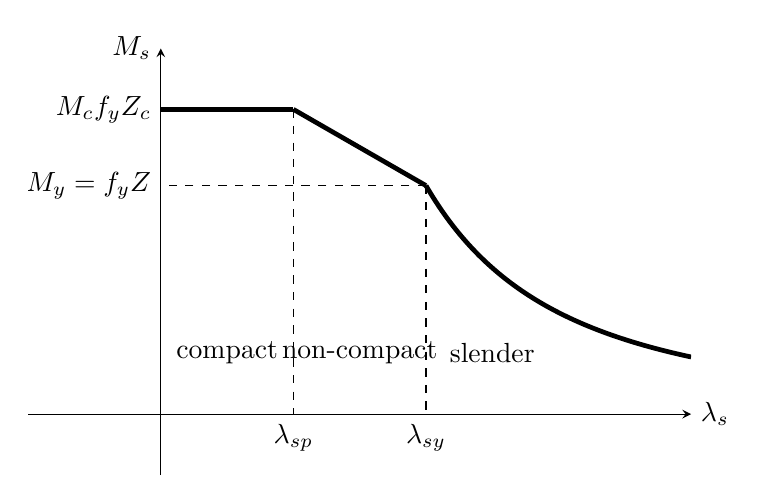
\begin{tikzpicture}[>=latex]
\begin{axis}[
width=10cm,
height=7cm,
xtick=\empty,
ytick=\empty,
axis x line=center,
axis y line=center,
xlabel={$\lambda_s$},
ylabel={$M_s$},
xlabel style={right},
ylabel style={left},
xmin=-1,xmax=4,ymin=-.2,ymax=1.2]
\addplot[line width=.6mm,domain=0:1,samples=100]{1};
\addplot[line width=.6mm,domain=1:2,samples=100]{-0.25*x+1.25};
\addplot[line width=.6mm,domain=2:4,samples=100]{3/x/x};
\draw[dashed](1,1)--(1,0)node[below]{$\lambda_{sp}$};
\draw[dashed](2,.75)--(2,0)node[below]{$\lambda_{sy}$};
\draw[dashed](1,1)--(0,1)node[left]{$M_cf_yZ_c$};
\draw[dashed](2,.75)--(0,.75)node[left]{$M_y=f_yZ$};
\node at(.5,.2){compact};
\node at(1.5,.2){non-compact};
\node at(2.5,.2){slender};
\end{axis}
\end{tikzpicture}